\documentclass[sigconf,authordraft]{acmart}

\usepackage{gensymb}

\AtBeginDocument{%
  \providecommand\BibTeX{{%
    \normalfont B\kern-0.5em{\scshape i\kern-0.25em b}\kern-0.8em\TeX}}}

\citestyle{acmauthoryear}

\begin{document}

\title{Application of Reinforcement Learning in NASA Swarmathon Competition}

\author{Rolando J. Nieves}
\email{rolando.j.nieves@knights.ucf.edu}
\authornotemark[1]
\affiliation{%
  \institution{University of Central Florida}
  \streetaddress{4000 Central Florida Blvd.}
  \city{Orlando}
  \state{Florida}
  \postcode{32816}
}

\renewcommand{\shortauthors}{Nieves}

\begin{abstract}
  The NASA Swarmathon competition domain provides an excellent proving ground
  for the implementation of multi-agent cooperative behavior using Reinforcement
  Learning (RL). This report documents the results of a study aimed at replacing
  the fixed, swarm-like logic offered as a baseline to competition entrants with
  a system that can be trained in a simulated environment prior to deployment
  onto an entrant's physical robots.
\end{abstract}

\begin{CCSXML}
  <ccs2012>
    <concept>
      <concept_id>10010147.10010178.10010219.10010220</concept_id>
      <concept_desc>Computing methodologies~Multi-agent systems</concept_desc>
      <concept_significance>500</concept_significance>
    </concept>
    <concept>
      <concept_id>10010147.10010257.10010258.10010261.10010275</concept_id>
      <concept_desc>Computing methodologies~Multi-agent reinforcement learning</concept_desc>
      <concept_significance>500</concept_significance>
    </concept>
  </ccs2012>
\end{CCSXML}

\ccsdesc[500]{Computing methodologies~Multi-agent systems}
\ccsdesc[500]{Computing methodologies~Multi-agent reinforcement learning}

\keywords{multi-agent systems,machine learning,reinforcement learning}

\begin{teaserfigure}
  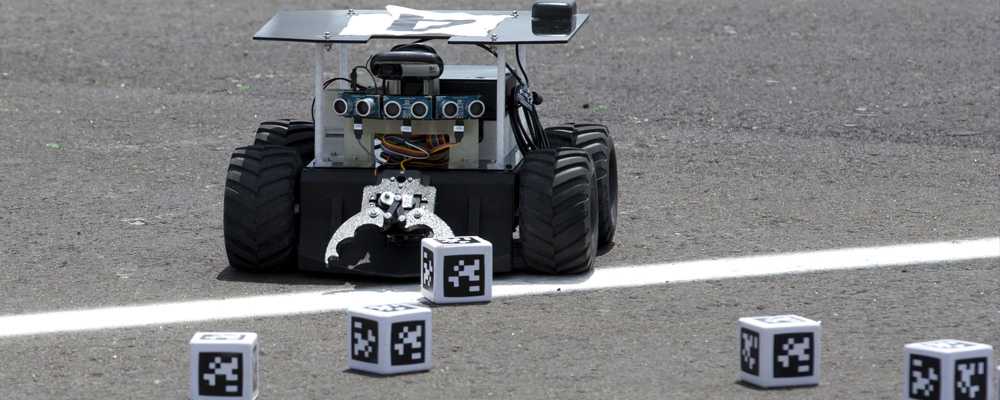
\includegraphics[width=\textwidth]{images/swarmathon-teaser.jpg}
  \caption{Montgomery College ``Swarmie'' in 2017 NASA Swarmathon}
  \Description{Image of a robotic member of the Montgomery College Swarmathon team entrant competing in NASA Swarmathon 2017}
  \label{fig:teaser}
\end{teaserfigure}

\maketitle

\section{Introduction}\label{sec:intro}
The study of applying Reinforcement Learning (RL) into cooperative multi-agent
systems remains a hot topic at the time of this writing. The topic's popularity
owes primarily to the fact that, unlike single agent RL, no single system
architecture has yet emerged as clearly superior among all available options.
Current architectural patterns such as Independent Learners (IL) and
Joint-Action Learners (JAL) exhibit traits that in some environments prove
quite beneficial. In other environments, however, these same traits represent
intolerable liabilities.

Thus, the search for a ``better mouse trap'' in the area of cooperating,
multi-agent RL has led to a proliferation of problem domains under which
methodology performance can be tested and quantified. From grid-world like
synthetic predator-prey scenarios, to more flexible environments like RoboCup
Simulated Soccer, these domains offer efficient ways to test theories. One
shortcoming of these problem domains, however, is the difficulty of implementing
any realized achievements into a physical domain.

The NASA Swarmathon problem domain offers an exciting opportunity for research
in this field. This is so because, combined with a robust simulation environment
based around the Robot Operating System (ROS) software suite, the domain offers
a clear path to implementation into physical robots participating in live
competition.

\section{Problem Domain}\label{sec:prob_domain}
NASA defines the Swarmathon competition environment using the following
elements:

\begin{itemize}
  \item A $16 \times 16$ or $32 \times 32$ meter square field where the
  competition takes place. The field size varies based on the round the
  competition is at.
  \item A swarm of three or six robots, with each robot labeled as a
  ``swarmie.''
  \item Up to 256, $2 \times 2 \times 2$ inch cubes bearing ``April Tag'' markers
  on all six faces, known as ``April Cubes.''
  \item A $1 \times 1$ meter square collection area within the competition
  field, known as a ``nest.''
\end{itemize}

During a competition round, a set of ``April Cubes'' are randomly strewn across
open areas of the competition field (i.e., no cubes initially start at
the ``nest''). The robotic swarm is then tasked with collecting the cubes onto
the ``nest.'' The periphery of the nest is labeled using another set of ``April
Tags,'' serving as a visual indicator for the robots. Collected cubes must be
in contact with the ``nest'' in order for them to count towards the team's
overall score.

Team members are not allowed contact or communication with the robots
(``swarmies'') during a round, leaving the robots to complete the task
leveraging their built-in sensor package and logic deployed to them prior to the
round. The elements that comprise the ``swarmie'' sensor package include the
following:

\begin{itemize}
  \item Three ultrasonic range finders able to detect obstacles up to 3 meters
  away. The sensors are located in front of the robot, and evenly distributed
  across a $60^{\circ}$ arc.
  \item One Inertial Measurement Unit (IMU) used to estimate robot orientation
  and, in combination with other sensors, robot pose in the fixed competition
  area.
  \item One camera emitting color $320 \times 240$ resolution images at about
  six frames per second (FPS).
  \item One Global Positioning Satellite (GPS) receiver emitting latitude and
  longitude readings that, in combination with other sensors, help establish the
  robot's pose in the competition area.
  \item One odometer emitting wheel movement that, in combination with other
  sensors, help establish the robot's pose in the competition area.
\end{itemize}

In order to combine, or ``fuse,'' several of the sensor readings into a complete
robot pose, the baseline software provided by NASA includes an Extended Kalman
Filter (EKF) pipeline that eventually produces the following pose information:

\begin{itemize}
  \item Cartesian $(x,y,z)$ position with (albeit mostly static) altitude.
  \item Yaw with respect to a fixed reference frame.
  \item Linear $(x,y)$ velocity.
  \item Angular velocity about the Yaw axis
  \item Linear $(x,y)$ acceleration. 
\end{itemize}

Given that the robots are four-wheeled traversing a flat area, linear velocity
and acceleration in the altitude $z$ axis, as well as angular position and
velocity about the Roll and Pitch axes is not calculated.

The NASA baseline software also includes computer vision facilities that, when
combined with the camera and robot pose calculations, are able to provide
information about any ``April Tags'' visible within the robot's field of view.
As stated previously, the ``April Cubes'' that the robots must gather are
labeled on all six faces with the aforementioned tags, as is the ``nest''
periphery where the robots must deposit the cubes.

The NASA baseline software is written in terms of the facilities and services
provided by ROS, particularly when it comes to communication. Software provided
by teams must run within ROS and only utilize the Publish-Subscribe system
provided with ROS for their communication needs. In addition, the NASA baseline
software provides a simulation environment that combines ROS Gazebo with 3D
models of the robots and sensor emulation. During a simulation session, the
communication traffic fed as input to the software components that combine to
implement a robot's logic is practically indistinguishable from traffic that
would be produced by the sensor package of a physical robot.

\section{Related Works}\label{sec:related_works}
Related works discussion.

\section{Methodology}\label{sec:methodology}
Methodology discussion.

\section{Experimental Results}\label{sec:results}
Results discussion.

\section{Conclusion}\label{sec:conclusion}
Final conclusion.

\bibliographystyle{ACM-Reference-Format}
\bibliography{swarmies_rl}

\end{document}
